% CircusTent Section

CircusTent

\begin{figure*}[!t]
\centering
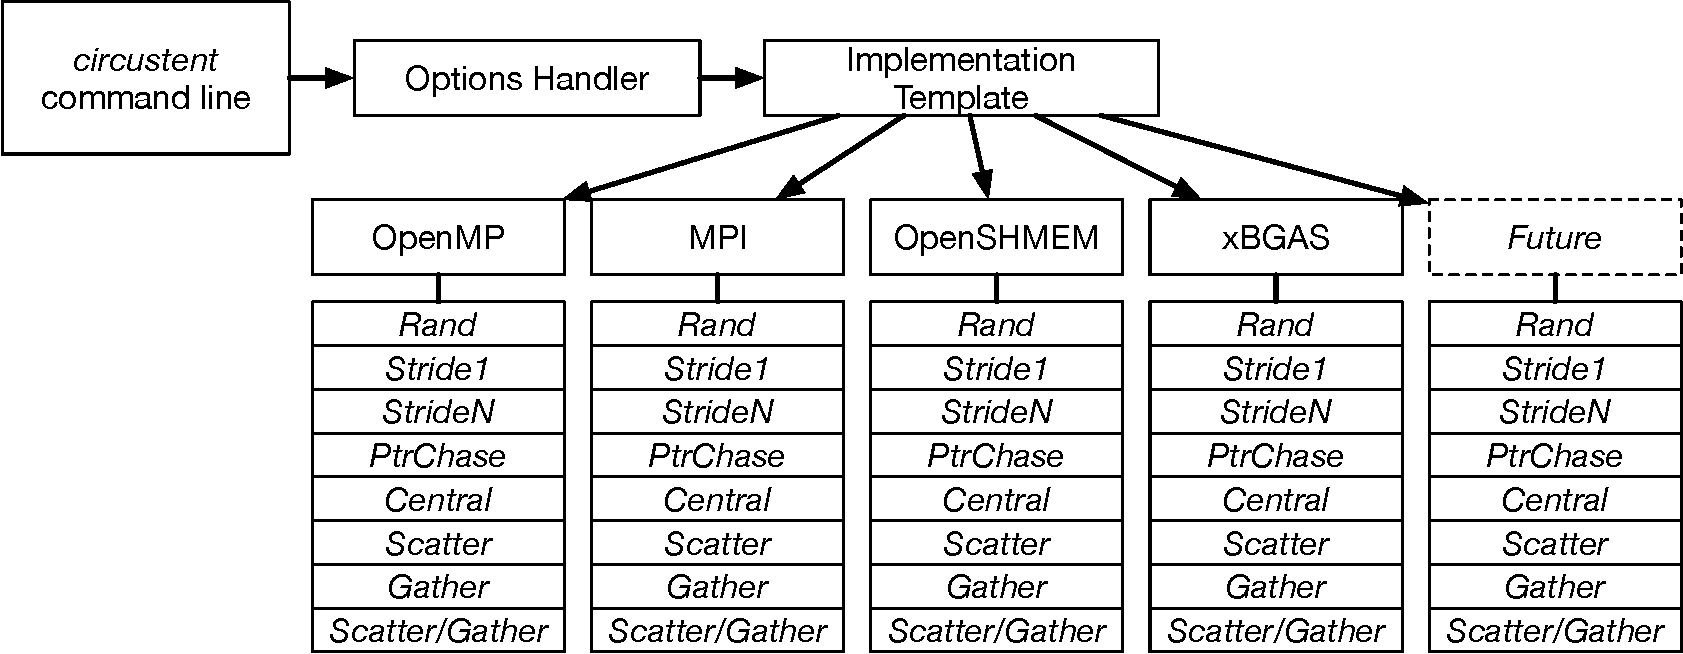
\includegraphics[width=5in]{figures/arch.pdf}
\caption{CircusTent Architecture}
\label{fig:ct_arch}
\end{figure*}

\subsection{Benchmark Overview}
\label{subsec:benchmark_overview}

\subsection{Programming Models}
\label{subsec:programming_models}

\subsection{Algorithms}
\label{subsec:algorithms}

\begin{algorithm}
\SetAlgoLined
\For{$i\gets0$ \KwTo $iters$ \KwBy $1$}{
AMO(ARRAY[IDX[i]])
}
\caption{Random Access Benchmark}
\label{alg:rand}
\end{algorithm}

\begin{algorithm}
\SetAlgoLined
\For{$i\gets0$ \KwTo $iters$ \KwBy $1$}{
AMO(ARRAY[i])
}
\caption{Stride-1 Benchmark}
\label{alg:s1}
\end{algorithm}

\begin{algorithm}
\SetAlgoLined
\For{$i\gets0$ \KwTo $iters$ \KwBy $stride$}{
AMO(ARRAY[i])
}
\caption{Stride-N Benchmark}
\label{alg:sn}
\end{algorithm}

\begin{algorithm}
\SetAlgoLined
\For{$i\gets0$ \KwTo $iters$ \KwBy $1$}{
start = AMO(IDX[start])
}
\caption{Pointer Chase Benchmark}
\label{alg:ptrchase}
\end{algorithm}

\begin{algorithm}
\SetAlgoLined
\For{$i\gets0$ \KwTo $iters$ \KwBy $1$}{
AMO(ARRAY[0])
}
\caption{Central Benchmark}
\label{alg:central}
\end{algorithm}

\begin{algorithm}
\SetAlgoLined
\For{$i\gets0$ \KwTo $iters$ \KwBy $1$}{
dest = AMO(IDX[i+1])\\
val = AMO(ARRAY[i])\\
AMO(ARRAY[dest], val) // ARRAY[dest] = val
}
\caption{Scatter Benchmark}
\label{alg:scatter}
\end{algorithm}

\begin{algorithm}
\SetAlgoLined
\For{$i\gets0$ \KwTo $iters$ \KwBy $1$}{
dest = AMO(IDX[i+1])\\
val = AMO(ARRAY[dest])\\
AMO(ARRAY[i], val) // ARRAY[i] = val
}
\caption{Gather Benchmark}
\label{alg:gather}
\end{algorithm}

\begin{algorithm}
\SetAlgoLined
\For{$i\gets0$ \KwTo $iters$ \KwBy $1$}{
src = AMO(IDX[i])\\
dest = AMO(IDX[i+1])\\
val = AMO(ARRAY[src])\\
AMO(ARRAY[dest], val) // ARRAY[dest] = val
}
\caption{Scatter/Gather Benchmark}
\label{alg:sg}
\end{algorithm}

\begin{table}
  \caption{Atomic Operation Distribution}
  \label{tab:amodistro}
  \begin{tabular}{cc}
    \toprule
    Benchmark&AMOs Per Iteration\\
    \midrule
   Rand & 1\\
   Stride-1 & 1\\
   Stride-N & 1\\
   Pointer Chase & 1\\
   Central & 1\\
   Scatter & 3\\
   Gather & 3\\
   Scatter/Gather & 4\\
  \bottomrule
\end{tabular}
\end{table}